\documentclass[tikz,border=10pt]{standalone}
\usepackage{tikz}
\usetikzlibrary{shapes.geometric, arrows, positioning, fit, shadows, matrix}

\begin{document}

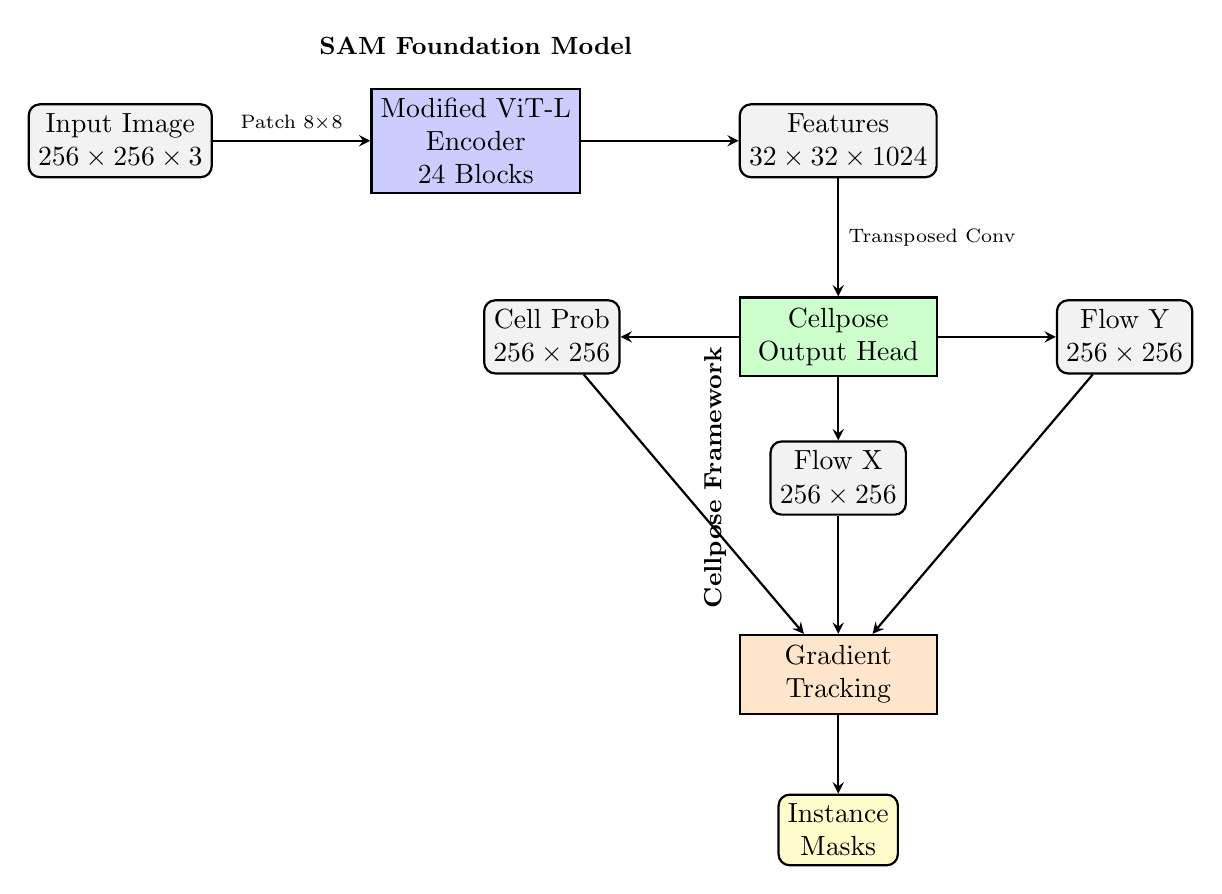
\begin{tikzpicture}[
    % Define styles
    encoder/.style={rectangle, draw, thick, fill=blue!20, minimum width=2.5cm, minimum height=1cm, align=center},
    decoder/.style={rectangle, draw, thick, fill=green!20, minimum width=2.5cm, minimum height=1cm, align=center},
    data/.style={rectangle, draw, thick, fill=gray!10, rounded corners, minimum height=0.8cm, align=center},
    arrow/.style={->, >=stealth, thick},
    dimension/.style={font=\scriptsize, above}
  ]

  % Input
  \node[data] (input) at (0,0) {Input Image\\$256 \times 256 \times 3$};

  % SAM Encoder
  \node[encoder, right=2cm of input] (vit) {Modified ViT-L\\Encoder\\24 Blocks};
  \draw[arrow] (input) -- node[above] {\scriptsize Patch 8×8} (vit);

  % Features
  \node[data, right=2cm of vit] (features) {Features\\$32 \times 32 \times 1024$};
  \draw[arrow] (vit) -- (features);

  % Cellpose Decoder
  \node[decoder, below=1.5cm of features] (decoder) {Cellpose\\Output Head};
  \draw[arrow] (features) -- node[right] {\scriptsize Transposed Conv} (decoder);

  % Flow outputs
  \node[data, left=1.5cm of decoder] (cellprob) {Cell Prob\\$256 \times 256$};
  \node[data, below=0.8cm of decoder] (dx) {Flow X\\$256 \times 256$};
  \node[data, right=1.5cm of decoder] (dy) {Flow Y\\$256 \times 256$};

  \draw[arrow] (decoder) -- (cellprob);
  \draw[arrow] (decoder) -- (dx);
  \draw[arrow] (decoder) -- (dy);

  % Mask reconstruction
  \node[decoder, below=1.5cm of dx, fill=orange!20] (recon) {Gradient\\Tracking};
  \draw[arrow] (cellprob) -- (recon);
  \draw[arrow] (dx) -- (recon);
  \draw[arrow] (dy) -- (recon);

  % Final output
  \node[data, below=1cm of recon, fill=yellow!20] (masks) {Instance\\Masks};
  \draw[arrow] (recon) -- (masks);

  % Annotations
  \node[above=0.3cm of vit, font=\small\bfseries] {SAM Foundation Model};
  \node[left=0.3cm of decoder, font=\small\bfseries, rotate=90] {Cellpose Framework};

\end{tikzpicture}

\end{document}
